% Options for packages loaded elsewhere
\PassOptionsToPackage{unicode}{hyperref}
\PassOptionsToPackage{hyphens}{url}
\PassOptionsToPackage{dvipsnames,svgnames*,x11names*}{xcolor}
%
\documentclass[
  12pt,
]{article}
\usepackage[]{mathpazo}
\usepackage{setspace}
\usepackage{amssymb,amsmath}
\usepackage{ifxetex,ifluatex}
\ifnum 0\ifxetex 1\fi\ifluatex 1\fi=0 % if pdftex
  \usepackage[T1]{fontenc}
  \usepackage[utf8]{inputenc}
  \usepackage{textcomp} % provide euro and other symbols
\else % if luatex or xetex
  \usepackage{unicode-math}
  \defaultfontfeatures{Scale=MatchLowercase}
  \defaultfontfeatures[\rmfamily]{Ligatures=TeX,Scale=1}
\fi
% Use upquote if available, for straight quotes in verbatim environments
\IfFileExists{upquote.sty}{\usepackage{upquote}}{}
\IfFileExists{microtype.sty}{% use microtype if available
  \usepackage[]{microtype}
  \UseMicrotypeSet[protrusion]{basicmath} % disable protrusion for tt fonts
}{}
\makeatletter
\@ifundefined{KOMAClassName}{% if non-KOMA class
  \IfFileExists{parskip.sty}{%
    \usepackage{parskip}
  }{% else
    \setlength{\parindent}{0pt}
    \setlength{\parskip}{6pt plus 2pt minus 1pt}}
}{% if KOMA class
  \KOMAoptions{parskip=half}}
\makeatother
\usepackage{xcolor}
\IfFileExists{xurl.sty}{\usepackage{xurl}}{} % add URL line breaks if available
\IfFileExists{bookmark.sty}{\usepackage{bookmark}}{\usepackage{hyperref}}
\hypersetup{
  colorlinks=true,
  linkcolor=blue,
  filecolor=Maroon,
  citecolor=Blue,
  urlcolor=Blue,
  pdfcreator={LaTeX via pandoc}}
\urlstyle{same} % disable monospaced font for URLs
\usepackage[margin=1in]{geometry}
\usepackage{graphicx}
\makeatletter
\def\maxwidth{\ifdim\Gin@nat@width>\linewidth\linewidth\else\Gin@nat@width\fi}
\def\maxheight{\ifdim\Gin@nat@height>\textheight\textheight\else\Gin@nat@height\fi}
\makeatother
% Scale images if necessary, so that they will not overflow the page
% margins by default, and it is still possible to overwrite the defaults
% using explicit options in \includegraphics[width, height, ...]{}
\setkeys{Gin}{width=\maxwidth,height=\maxheight,keepaspectratio}
% Set default figure placement to htbp
\makeatletter
\def\fps@figure{htbp}
\makeatother
\setlength{\emergencystretch}{3em} % prevent overfull lines
\providecommand{\tightlist}{%
  \setlength{\itemsep}{0pt}\setlength{\parskip}{0pt}}
\setcounter{secnumdepth}{-\maxdimen} % remove section numbering
\usepackage{hyperref}
\usepackage[]{natbib}
\bibliographystyle{plainnat}

\author{}
\date{\vspace{-2.5em}}

\begin{document}

\setstretch{1}
\begin{flushright} 
    \end{flushright}
    \begin{center} \textbf{Parlr: Parallelized Record Linkage in R}
    
    Brian Kundinger

    \end{center}

\hypertarget{introduction}{%
\subsection{Introduction}\label{introduction}}

Record linkage is the task of identifying duplicate records across
multiple data sources. This task is straightforward when provided unique
identifiers or highly reliable information, but becomes difficult when
data sources are plagued with error. Additionally, many record linkage
tasks are large in nature, and many existing methods are too
computational intensive to be used in practice. In this paper, we
propose a Bayesian model for record linkage that is amenable to parallel
computing, hashing techniques and efficient storage mechanisms, that is
scalable to large linkage tasks.

The proposed method is inspired by the ``Beta Record Linkage'' method
proposed by Mauricio Sadinle's 2017 ``Bayesian Estimation of Bipartite
Matching for Record Linkage''. As such, we demonstrate our method
through a comparison of our methods against Sadinle's on the simulation
study he designed and the El Salvador homocide case study he utilized.
We include one additional simulation study to demonstrate the power of
our method on large datasets. In what follows, Section 2 describes
previous work in record linkage that lays the foundation for our method,
Section 3 provides our model and the Gibbs sampler used for posterior
inference, and Section 4 describes strategies used for more efficient
and scalable implementation. Then, Sections 5 and 6 demonstrate the
method through simulations and a case study. Lastly, our discussion
highlights open questions in the record linkage liturature and motivates
future work.

\hypertarget{related-work}{%
\subsection{Related Work}\label{related-work}}

Most record linkage techniques are derived from the seminal 1969 paper
by Fellegi and Sunter: ``A Theory for Record Linkage''. The defining
characteristic of their model was to transform the sets of records,
which often contain text data that is difficult to model, into sets of
comparison vectors governed by parameters that can be more easily
estimated. Concretely, if files \(A\) and \(B\) have \(n_A\) and \(n_B\)
records respectively, and if the files share \(F\) fields in common upon
which to base the linkage, the Fellegi and Sunter approach generates a
\(n_A n_B \times F\) matrix \(\Gamma\), which contains similarity scores
between each pair of records across datasets. We say \(\gamma_{ij}\) is
the comparison vector for record \(i \in A\) and record \(j \in B\),
with \(\gamma_{ij}^f\) providing their similarity score on the
\(f^{th}\) field. For ease of modeling and computation, we restrict
these similarity scores to be discrete, ordinal variables, and the
construction of these is left to the modeler. It is common to use use
binary 0-1 variables to indicate exact matching, and 0-1-2 variables to
provide an option for partial matching. For text data, we calculate
similarity based on Levenstein distance or some other text similarity
score, and bin these scores to integers for use in the model.

The likelihood in the original Fellegi Sunter model is a mixture model
through which each record pair is independently classified as a match or
nonmatch. This independent classification often leads to sets of matches
that break expectations of transisitivity, and Jaro devised an procedure
to reduce a set of conflicting matches to the mostly likely set of
one-to-one matchings. One key strength of Sadinle's \texttt{BRL} is that
it is garunteed to produce a set of bipartite matchings that respect
one-to-one assumptions--without the need for any post-hoc procedures.
Specifically, in each iteration of his Gibbs sampler, he considers each
record \(j\in B\), removes from consideration the records \(i\in A\)
that have already been matched, and then samples a potential link.
However, accounting for these dependencies throughout the linkage
process is computationally burdensome, leaving \texttt{BRL} only
suitable for small to moderate linkage problems.

Outside of the Fellegi-Sunter framework, some researchers have developed
methods that model the data directly, not a derived set of comparison
vectors. As an early example, Steorts et al 2016 produced
\texttt{blink}, which had the advantage of a computational complexity
that grew linearly with the data (as opposed to quadratically within
Fellegi Sunter), but was plagued with slow mixing times and was unable
to incorporate text data. Later, Steorts et al 2020 improved on this
method with \texttt{dblink}, which was able to simulate text data within
its Gibbs sampler by drawing from an empirical distribution, and
remedied its slow mixing through a probabilistic blocking approach.
However, this method remains computationally intensive and requires
distributed computing to manage even moderate linkage problems in
acceptable time. Because these methods fall outside of the
Fellegi-Sunter framework, we do not consider them further in this paper.

\hypertarget{notation-and-assumptions}{%
\subsection{Notation and Assumptions}\label{notation-and-assumptions}}

Our notation and assumptions closely follow those of Sadinle. Denote two
files as \(A\) and \(B\), with \(n_A\) and \(n_B\) records respectively,
and with records indexed as \(i \in \{1, \ldots, n_A\}\) in \(A\) and
\(j \in \{1, \ldots, n_B\}\) in \(B\). Without loss of generality, label
the files such that \(n_A \geq n_B\). We also assume there are no
duplicates within files, only across. For each record pair under
consideration, we generate a comparison vector
\(\boldsymbol{\gamma}_{ij} = \{\gamma_{ij}^1, \ldots, \gamma_{ij}^F\}\),
where \(F\) is the number of fields used in the linkage and each
\(\gamma_{ij}^f\) takes on a value \(l \in \{1, \ldots, L_f\}\)
indicating the level agreement between the two records on a specified
field.

To indicate matching status, we adopt the \emph{linkage structure
parameter} \(\mathbf{Z} = (Z_1, \ldots, Z_{n_B})\) from Sadinle 2017,
defined as \[Z_j=\begin{cases} 
    i,  & \text{if records } i\in A \text{ and } j\in B \text{ refer to the same entity}; \\
    n_A + 1,  & \text{if record } j\in B \text{ does not have a match in file } A; \\
\end{cases}\] This provides more memory efficient storage for the
linkage information than a \(n_A \times n_B\) sparse matrix of
indicators.

Following the Fellegi Sunter framework, we define
\(m^{fl}:= P(\gamma_{ij}^f = l |Z_j = i)\) to be the probability of
observing agreement level \(l\) in field \(f\) for records \(i\) and
\(j\) given that the records are a match, and similarly define
\(u^{fl}:= P(\gamma_{ij}^f = l |Z_j \neq i)\), for non-matches. We also
adopt Fellegi and Sunter's conditionally independent fields assumption
that the level of agreement on one field is independent of the level of
agreement on another. Though this assumption is often not reasonable
(for example, first name and gender are two clearly dependent fields),
but it is common within the record linkage literature and generally
leads to models that perform well in practice; see discussion for
further remarks. Lastly, we define \(\lambda\) to be the (marginal)
probability that some record \(j \in B\) has a match in \(A\).

Wherever possible, we reserve superscripts for denoting field and level,
while reserving subscripts for record indices. For example,
\(\mathbf{m}^f = (m^{f1}, \ldots, m^{fL_f})\) is the probability
distribution governing field \(f\) for matching records, and
\(\mathbf{m}_{ij}= \prod_{f=1}^{F}\prod_{l=1}^{L_f} \left(m^{fl}\right)^{\mathbf{1}_{\gamma_{ij}^f = l}} = P(\boldsymbol{\gamma}_{ij}|Z_j = i)\)
is product of the relevant of the appropriate \(\mathbf{m}\) parameters
for record pair \((i,j)\). We hope that these conventions avoid
overloaded notation in the likelihood and subsequent derivations.

\hypertarget{model-specification}{%
\subsection{Model Specification}\label{model-specification}}

For fields \(f \in \{1, \ldots, F\}\) and levels
\(l\in \{1, \ldots, L_f\}\) we adopt the following likelihood and prior
distributions.

\[P(\Gamma|\mathbf{Z}, \mathbf{m}, \mathbf{u}, \lambda) =\prod_{j=1}^{n_B}  \prod_{i=1}^{n_A}\mathbf{m}_{ij}^{\mathbf{1}_{z_j = i}}\mathbf{u}_{ij}^{\mathbf{1}_{z_j \neq i}}\]

\[\mathbf{m^{f}} \sim \text{Dirichlet}(\alpha^{f1}, \ldots, \alpha^{fL_f})\]
\[\mathbf{u^{f}} \sim \text{Dirichlet}(\beta^{f1}, \ldots, \beta^{fL_f})\]
\[Z_j | \lambda =
\begin{cases} 
    \frac{1}{n_A}\lambda  & z_j \leq n_A; \\
     1-\lambda &  z_j  = n_A + 1 \\
\end{cases}\]

\[\lambda \sim \text{Beta}(\alpha_{\lambda}, \beta_{\lambda}) \] The
prior for \(Z_j\) has equal probability of matching to all records
\(i\in A\), and non-matching probability governed by \(\lambda\).
Therefore a \(\lambda \sim \text{Beta}(1, 1)\) corresponds to a prior
belief that nonmatches and matches are equally likely, and a
\(\lambda \sim \text{Beta}(1, \frac{1}{n_A})\) prior corresponds to a
uniform prior on the labeling of \(\mathbf{Z}\).

Here the reader should the relationship between our proposed model and
that of Sadinle 2017. In his model, Sadinle constructs a prior
distribution on the entire \(\mathbf{Z}\) vector, which induces a Gibbs
sampler that strictly enforces one-to-one matching. In particular, this
sampler removes previously matches records from the set of candidate
records when sampling \(Z_j\), creating a dependency that makes the
sampler \emph{inherently serial}. We however use independent priors for
each \(Z_j\), thereby weakening the one-to-one requirement; our sampler
does ensure that each record in \(B\) can be matched to at most one
record in \(A\), but allows for the possiblity that multiple records in
\(B\) match to the same record in \(A\). We explore the ramifications of
this distinction with the El Salvador case study. With this change,
components of the \(\mathbf{Z}\) vector can be computed in parallel,
allowing for significant computational gains. More importantly, since
only the agreement pattern of \(Z_j\) is used for calculations within
the Gibbs sampler, and not the particular record label, we can conduct
this sampling only at the level of the unique agreement patterns,
offering even more computational savings. This will be explained further
in \textcolor{red}{Section XX}.

\hypertarget{posterior-sampling}{%
\subsection{Posterior Sampling}\label{posterior-sampling}}

We work with the following factorization of the joint distribution:

\[p(\Gamma, \mathbf{Z}, \mathbf{m}, \mathbf{u}, \lambda) = p(\Gamma|\mathbf{Z}, \mathbf{m}, \mathbf{u}) p(\mathbf{Z} | \lambda) p(\mathbf{m}, \mathbf{u}) p(\lambda)\]

This factorization leads to following Gibbs Sampler:

\underline{Sample $\mathbf{m}^{(s+1)}$ $\mathbf{u}^{(s+1)}|\Gamma, \mathbf{Z}^{(s)}$:}
The \(\mathbf{m}\) and \(\mathbf{u}\) parameters are updated through
standard multinomial-dirichlet mechanics. Thus we have

\[\mathbf{m}^f|\mathbf{Z}, \Gamma \sim \text{Dirichlet}(\alpha^{f1}(\mathbf{Z}), \ldots, \alpha^{fL_f}(\mathbf{Z}))\]
\[\mathbf{u}^f|\mathbf{Z}, \Gamma \sim \text{Dirichlet}(\beta^{f1}(\mathbf{Z}), \ldots, \beta^{fL_f}(\mathbf{Z}))\]
where
\(\alpha_{fl}(\mathbf{Z})= \sum_{i,j} \mathbf{1}_{obs(\gamma_{ij}^f)}\mathbf{1}_{\gamma_{ij}^f = l} \mathbf{1}_{z_j = i}\)
and
\(\beta_{fl}(\mathbf{Z})= \mathbf{1}_{obs(\gamma_{ij}^f)}\mathbf{1}_{\gamma_{ij}^f = l} \mathbf{1}_{z_j \neq i}\).

\underline{Sample $\lambda^{(s+1)}|\mathbf{Z}^{(s)}$:} As a function of
\(\lambda\), the linkage structure parameter \(\mathbf{Z}\) is sequence
of successes (when \(z_j < n_A + 1\)) and failures (when
\(z_j = n_A + 1\)), and therefore
\(p(\mathbf{Z}|\lambda) = \mathcal{L}(\lambda|\mathbf{Z})\) is
determined only by the number of duplicates
\(D = \sum_{i=1}^{n_B}\mathbf{1}_{z_j < n_A + 1}\) encoded by
\(\mathbf{Z}\). Thus we have

\[p(\lambda | \mathbf{Z}) \propto p(\mathbf{Z}|\lambda)p(\lambda)\]
\[\propto \lambda^D (1-\lambda)^{n_B - D} \lambda^{\alpha_{\lambda} -1} (1-\lambda)^{\beta_{\lambda} -1}\]
\[ \propto \lambda^{D + \alpha_{\lambda} - 1} (1-\lambda)^{n_B - D + \beta_{\lambda} -1}\]
\[\implies \lambda^{(s+1)}|\mathbf{Z}^{(s+1)} \sim \text{Beta}(D + \alpha_{\lambda}, n_B - D + \beta_{\lambda})\]

\underline{Sample $\mathbf{Z}^{(s+1)}|\Gamma, \mathbf{m}^{(s+1)}, \mathbf{u}^{(s+1)}, \lambda^{(s+1)}$:}
Because we sample \(Z_j\) independently of all other \(Z_{j'}\), we use
only the full conditional for an individual \(Z_j\). Let \(\Gamma_{.j}\)
denote the set of \(n_A\) comparison vectors with \(j \in B\), and note
that as a function of \(Z_j\), the likelihood
\(p(\Gamma_{.j}|Z_j, \mathbf{m}, \mathbf{u}) = \mathcal{L}(Z_j|\Gamma_{.j}, \mathbf{m}, \mathbf{u})\)
is a discrete distribution with probabilities proportional to

\begin{align*}
p(\Gamma_{.j}|Z_j = z_j, \mathbf{m}, \mathbf{u}) &\propto \prod_{i=1}^{n_A}\mathbf{m}_{ij}^{\mathbf{1}_{z_j = i}}\mathbf{u}_{ij}^{\mathbf{1}_{z_j \neq i}}\\
&\propto \prod_{i=1}^{n_A}\left(\frac{\mathbf{m}_{ij}}{\mathbf{u}_{ij}}\right)^{\mathbf{1}_{z_j = i}} && \text{By dividing through by} \prod_{i = 1}^{n_A}\mathbf{u}_{ij}\\
&=
\begin{cases} 
    w_{ij}  & z_j \leq n_A; \\
    1 &  z_j  = n_A + 1 \\
\end{cases}\\
\end{align*}

where
\(w_{ij} = \frac{\mathbf{m}_{ij}}{\mathbf{u}_{ij}} = \frac{P(\boldsymbol{\gamma_{ij}}|Z_j = i)}{P(\boldsymbol{\gamma_{ij}} |Z_j \neq i)}\).
The interested reader should note that these are precisely the
likelihood ratios used in the Fellegi-Sunter model to classify matches
and non-matches, and we therefore refer to \(w_{ij}\) as the
\emph{Fellegi Sunter weights}.

With the likelihood in this form, we can derive the full conditional
\[p(Z_j|\Gamma_{.j}, \mathbf{m} ,\mathbf{u}, \lambda) \propto p(\Gamma_{.j}| Z_j, \mathbf{m} ,\mathbf{u}) P(Z_j|\lambda)\]

\[\propto \left(\sum_{i=1}^{n_A}w_{ij}\mathbf{1}_{z_j = i} + \mathbf{1}_{z_j = n_A + 1}\right)\left(\lambda\sum_{i=1}^{n_A}\frac{1}{n_A}\mathbf{1}_{z_j = i} + (1-\lambda)\mathbf{1}_{z_j = n_A + 1}\right)\]
\[= \frac{\lambda}{n_A}\sum_{i=1}^{n_A}w_{ij}\mathbf{1}_{z_j = i} + (1-\lambda)\mathbf{1}_{z_j = n_A + 1} \]
\[ \implies Z_j^{(s+1)} | \mathbf{m}, \mathbf{u}, \Gamma, \lambda \propto
\begin{cases} 
    \frac{\lambda}{n_A}w_{ij}   & z_j \leq n_A; \\
     1-\lambda &  z_j  = n_A + 1 \\
\end{cases}\]

In order to make fair comparisons against the Sadinle 2017 model, we
integrate over the posterior of \(\lambda\) and rearrange terms to
produce the final full conditional:

\[p\left(Z_j^{(s+1)}  = i| \mathbf{m}, \mathbf{u}, \mathbf{Z^{(s)}}\right) \propto
\begin{cases} 
    w_{ij}  & i \leq n_A; \\
     n_A \frac{n_B - D + \beta_{\lambda}}{D + \alpha_{\lambda}} & i  = n_A + 1 \\
\end{cases}\]

\hypertarget{bayes-estimate}{%
\subsection{Bayes Estimate}\label{bayes-estimate}}

(Adapt from Sadinle)

Since our Gibbs procedure does not strictly enforce one-to-one matching,
it is possible for the final Bayes estimate to link multiple records in
\(B\) to one record in \(A\). The modeler can either report both such
matches (with their respective posterior match probabilities), or
resolve these conflicts by accepting only the match with highest
posterior probability. Rigorous proof of this resolution procedure is
deferred to future work.

\hypertarget{efficient-computation}{%
\section{Efficient Computation}\label{efficient-computation}}

Broadly speaking, we increase our computational efficiency by
recognizing that record pairs contribute to posterior calculations only
through the agreement pattern of the \(\gamma_{ij}\) vector. Let
\(\mathcal{H}\) be the set of unique agreement patterns in the data, let
\(P\) denote the total number of unique agreement patterns. Note that
\(P\) is bounded above by \(\prod_{f=1}^F L_f\), and that this bound
does not scale with \(n_A\) or \(n_B\). Prior to processing the data, we
identify all \(P\) patterns in \(\mathcal{H}\) and enumerate them
\(h_1, \ldots, h_P\). When the \((i,j)\) pair exhibits the \(p^{th}\)
agreement pattern, we say \((i,j) \in h_p\). Wherever possible, we
conduct calculations over these \(P\) agreement patterns rather than the
\(n_A \times n_B\) record pairs.

\hypertarget{data-representation-hashing-and-storage}{%
\subsection{Data Representation, Hashing, and
Storage}\label{data-representation-hashing-and-storage}}

The classic Fellegi Sunter method represents the \(\gamma_{ij}\)
comparison vector as vector of length \(F\), with each component
\(\gamma_{ij}^f\) taking on values in \(\{0, \ldots, L_f - 1\}\). To
ease computations, we instead represent the comparison as a
concatenation of \(F\) many binary indicator vectors of lengths \(L_f\).
For example, if \(L_1 = L_2 = 2\) and \(L_3 = 3\), then
\(\gamma_{ij} = (1, 0, 2)\) under the classical framework becomes
\(\gamma_{ij} = (0, 1, 1, 0, 0, 0, 1)\) under our framework. This is a
bijective transformation that does not change the meaning of the data,
but this representation will ease calculations and posterior updates.

In the classic Fellegi Sunter framework, \(\Gamma\) is a
\(n_A n_B \times F\) matrix, with each row providing the comparison
vector for a different \((i,j)\) pair. We however do not store these
comparison vectors themselves, but instead only a hashed value
corresponding to the agreement pattern of the \((i, j)\) pair. We store
this information in a nested list \(\tilde{\Gamma}\) where the
\(p^{th}\) component of the \(j^{th}\) list contains a vector of records
in \(A\) that share agreement pattern \(p\) with record \(j \in B\). For
each \(p\), we also calculate
\(H_p = \sum_{i=1}^{n_A}\sum_{j=1}^{n_B} \mathbf{1}_{(i,j) \in h_p}\),
the total instances of agreement pattern \(p\) throughout the data, and
also for each \(j\), we calculate
\(H_{p_j} = \sum_{i=1}^{n_A} \mathbf{1}_{{(i,j) \in h_p}}\) the
instances of agreement pattern \(p\) among the comparison vectors
between record \(j \in B\) and each of the \(n_A\) records in \(A\).

For large data, we can partition the two datasets \(A\) and \(B\) into
smaller blocks \(\{A_m\}\) and \(\{B_m\}\) for more manageable
computations. On a single machine, we can read-in data sequentially,
conduct hashing, collect results, and delete the original data from
memory before continuing with the next chunk of data. With multiple
cores or multiple machines, this can be done in parallel. Storing this
hashed information still becomes burdensome for large data, but this
hashing method greatly expands the capabilities of the Fellegi-Sunter
framework.

The hashing procedure described above considerably reduces the memory
needed to store the comparison information: instead of storing
\(n_A \times n_B\) comparison vectors, which are relatively long under
either the Fellegi Sunter or our modified framework, we only store the
\(P\) unique vectors, and then \(n_A \times n_B\) scalar quantities
relating record pairs to those vectors. However, even storing these
\(n_A \times n_B\) scalar labels can become burdensome with large data.
Worse, the overwhelming majority of these labels relate to record pairs
that are clear non-matches.

To address this, we propose a new strategy called \emph{storage
efficient indexing} (SEI). In standard indexing, the modeler decides a
certain criteria that they expect all true matching pairs to satisfy,
and a priori label any record pairs that do not meet that criteria as
non-matching. For example, one might only consider pairs with a certain
similarity score on a field deemed to be important (like first name), or
only pairs with exact matching on a specified number of fields. While
generally chosen to be be quite loose, establishing these criteria
requires knowledge of the problem and invites room for human error. We
propose a method of reducing the comparison space (and reducing storage
requirements) without these drawbacks. Note that all records of the same
agreement pattern have the same probability when sampling \(Z_j\).
Therefore we know that records belonging to an \(h_p\) such that
\(H_{p_j}\) is large are very unlikely to be sampled consistently enough
to be deemed a match through the Bayes estimate, even without
considering the form of the agreement pattern itself. In random
indexing, rather than store all of these unlikely record labels, we
choose to store only a small number \(R\) of them. Posterior
calculations still attribute the appropriate weight to all records
through the summary statistics \(H_{p_j}, H_p^m\), and \(H_p^u\). Rather
than storing \(n_A \times n_B\) record labels, SEI allows us to store at
most \(n_B \times P \times R\) labels, regardless of how large \(n_A\)
is. Coupled with the partitioning strategy for creating comparison
vectors, this greatly expands the size of the linkage tasks we can
undertake.

\hypertarget{gibbs-sampling}{%
\subsection{Gibbs Sampling}\label{gibbs-sampling}}

\underline{Updating $\mathbf{m}$ and $\mathbf{u}$:} After receiving
matching statuses from \(\mathbf{Z}\), the Sadinle method calculates
\(\alpha_{fl}(\mathbf{Z})\) and \(\beta_{fl}(\mathbf{Z})\) for each
field and level. This constitutes \(2 \times \sum L_f\) many summations
over \(n_A \times n_B\) quantities, and becomes computationally
burdensome with large data. In contrast, we recognize that each unique
agreement pattern contributes to the posterior \(\alpha(\mathbf{Z})\)
and \(\beta(\mathbf{Z})\) vectors in the same way. In fact, if we denote
\(H_p^m = \sum_{j=1}^{n_B} \mathbf{1}_{(Z_j, j) \in h_p}\) to be the
number of matching record pairs with agreement pattern \(p\), then the
contribution of pairs of pattern \(p\) to the \(\alpha(\mathbf{Z})\)
vector is simply \(H_p^m \times h_p\). Thus our posterior update for
\(\alpha\) is simply
\(\alpha(\mathbf{Z}) = \alpha_0 + \sum_{p=1}^P H_p^m \times h_p\). Then,
we can easily calculate \(H_p^u\), the number of nonmatching record
pairs of agreement pattern \(p\), by subtracting the number of matching
pairs from the total present in the data; that is
\(H_p^u = H_p - H_p^m\). From this, we can update our \(\beta\)
parameter through
\(\beta(\mathbf{Z}) = \beta_0 + \sum_{p=1}^P H_p^u \times h_p\). Note
that these constitute \(P\) many summations over \(n_B\) quantities, and
thus avoid the \(n_A \times n_B\) summation from the original method.

\underline{Updating $\mathbf{Z}$:} Although sampling \(Z_j\) from a the
full conditional provided earlier is conceptually straightforward, it
becomes computational burdensome when \(n_A\) is larger. The reader can
confirm that sampling a value from a large set of unequal probabilities
becomes difficult in most programming languages. To speed up
computation, we break this sampling step into two simpler steps. First,
we calculate the Fellegi Sunter weight \(w_{h_p}\) associated with each
unique pattern and sample the agreement pattern between \(j\) and its
potential match. Second, we sample the record label uniformly among
records associated with that agreement pattern for that particular
\(j\in B\). More concretely, define \(h(Z_j)\) to be the agreement
pattern between \(j\) and its potential match, and say
\(h(Z_j) = h_{P+1}\) when \(Z_j = n_A + 1\). Then,

\[h\left(Z_j^{(s+1)}\right) | \mathbf{m}, \mathbf{u}, \mathbf{Z^{(s)}} \propto
\begin{cases} 
    w_{h_p}\times H_{p_j}  & p \leq P; \\
     n_A \frac{n_B - D + \beta_{\lambda}}{D + \alpha_{\lambda}} &   p = P + 1 \\
\end{cases}\]

Lastly, we recognize that all posterior updates are governed by the
agreement patterns of the record pairs rather than the record labels
themselves. Thuse We complete the entire Gibbs procedure at the level of
the \(P\) agreement patterns. After, we can back-fill the records
corresponding to the agreement patterns by sampling uniformly at random
among candidate records stored in \(\tilde{\Gamma}\). Sampling uniformly
is computational simple even for large sets of candidate records, but
this step can also be parallelized when working with large data.

\hypertarget{simulation-study-1---accuracy}{%
\section{Simulation Study 1 -
Accuracy}\label{simulation-study-1---accuracy}}

In his 2017 paper, Sadinle demonstrated the accuracy of his method by
running \texttt{BRL} on simulated pairs of files with differing levels
of errors and overlap. Each file consists of first name, last name,
gender, postal code, age, and occupation, and following Sadinle's
implementation, we use only four fields for the linkage process: both
names, age, and occupation. Similarity scores for the names are binned
into three levels according the default settings for the
\texttt{compareRecords} function in the \texttt{BRL} package, and age
and occupation similarity scores are binary for exact matching. We use
flat priors for all \(\mathbf{m}\) and \(\mathbf{u}\) parameters, and
run the Gibbs sampler for 1000 iterations, with the first 100 discarded
as burn-in.

Comparing our method against \texttt{BRL} on these same simulated
datasets, we find that our method only has weakened performance in the
most extreme scenario of very high errors and very high overlap across
files. We use the following measures of accuracy in our analysis:
although using only recall and precision is common in the literature, we
find it useful to have a single metric the gauge overall performance,
and thus also include F measure.

\[\text{Recall} = \frac{\text{Matches Correctly Identified}}{\text{True Matches in Data}}\]
\[\text{Precision} = \frac{\text{Declared Matches}}{\text{True Matches in Data}}\]
\[\text{F-Measure} = 2\left(\frac{\text{Recall} \times \text{Precision}}{\text{Recall} + \text{Precision}}\right)\]

\begin{center}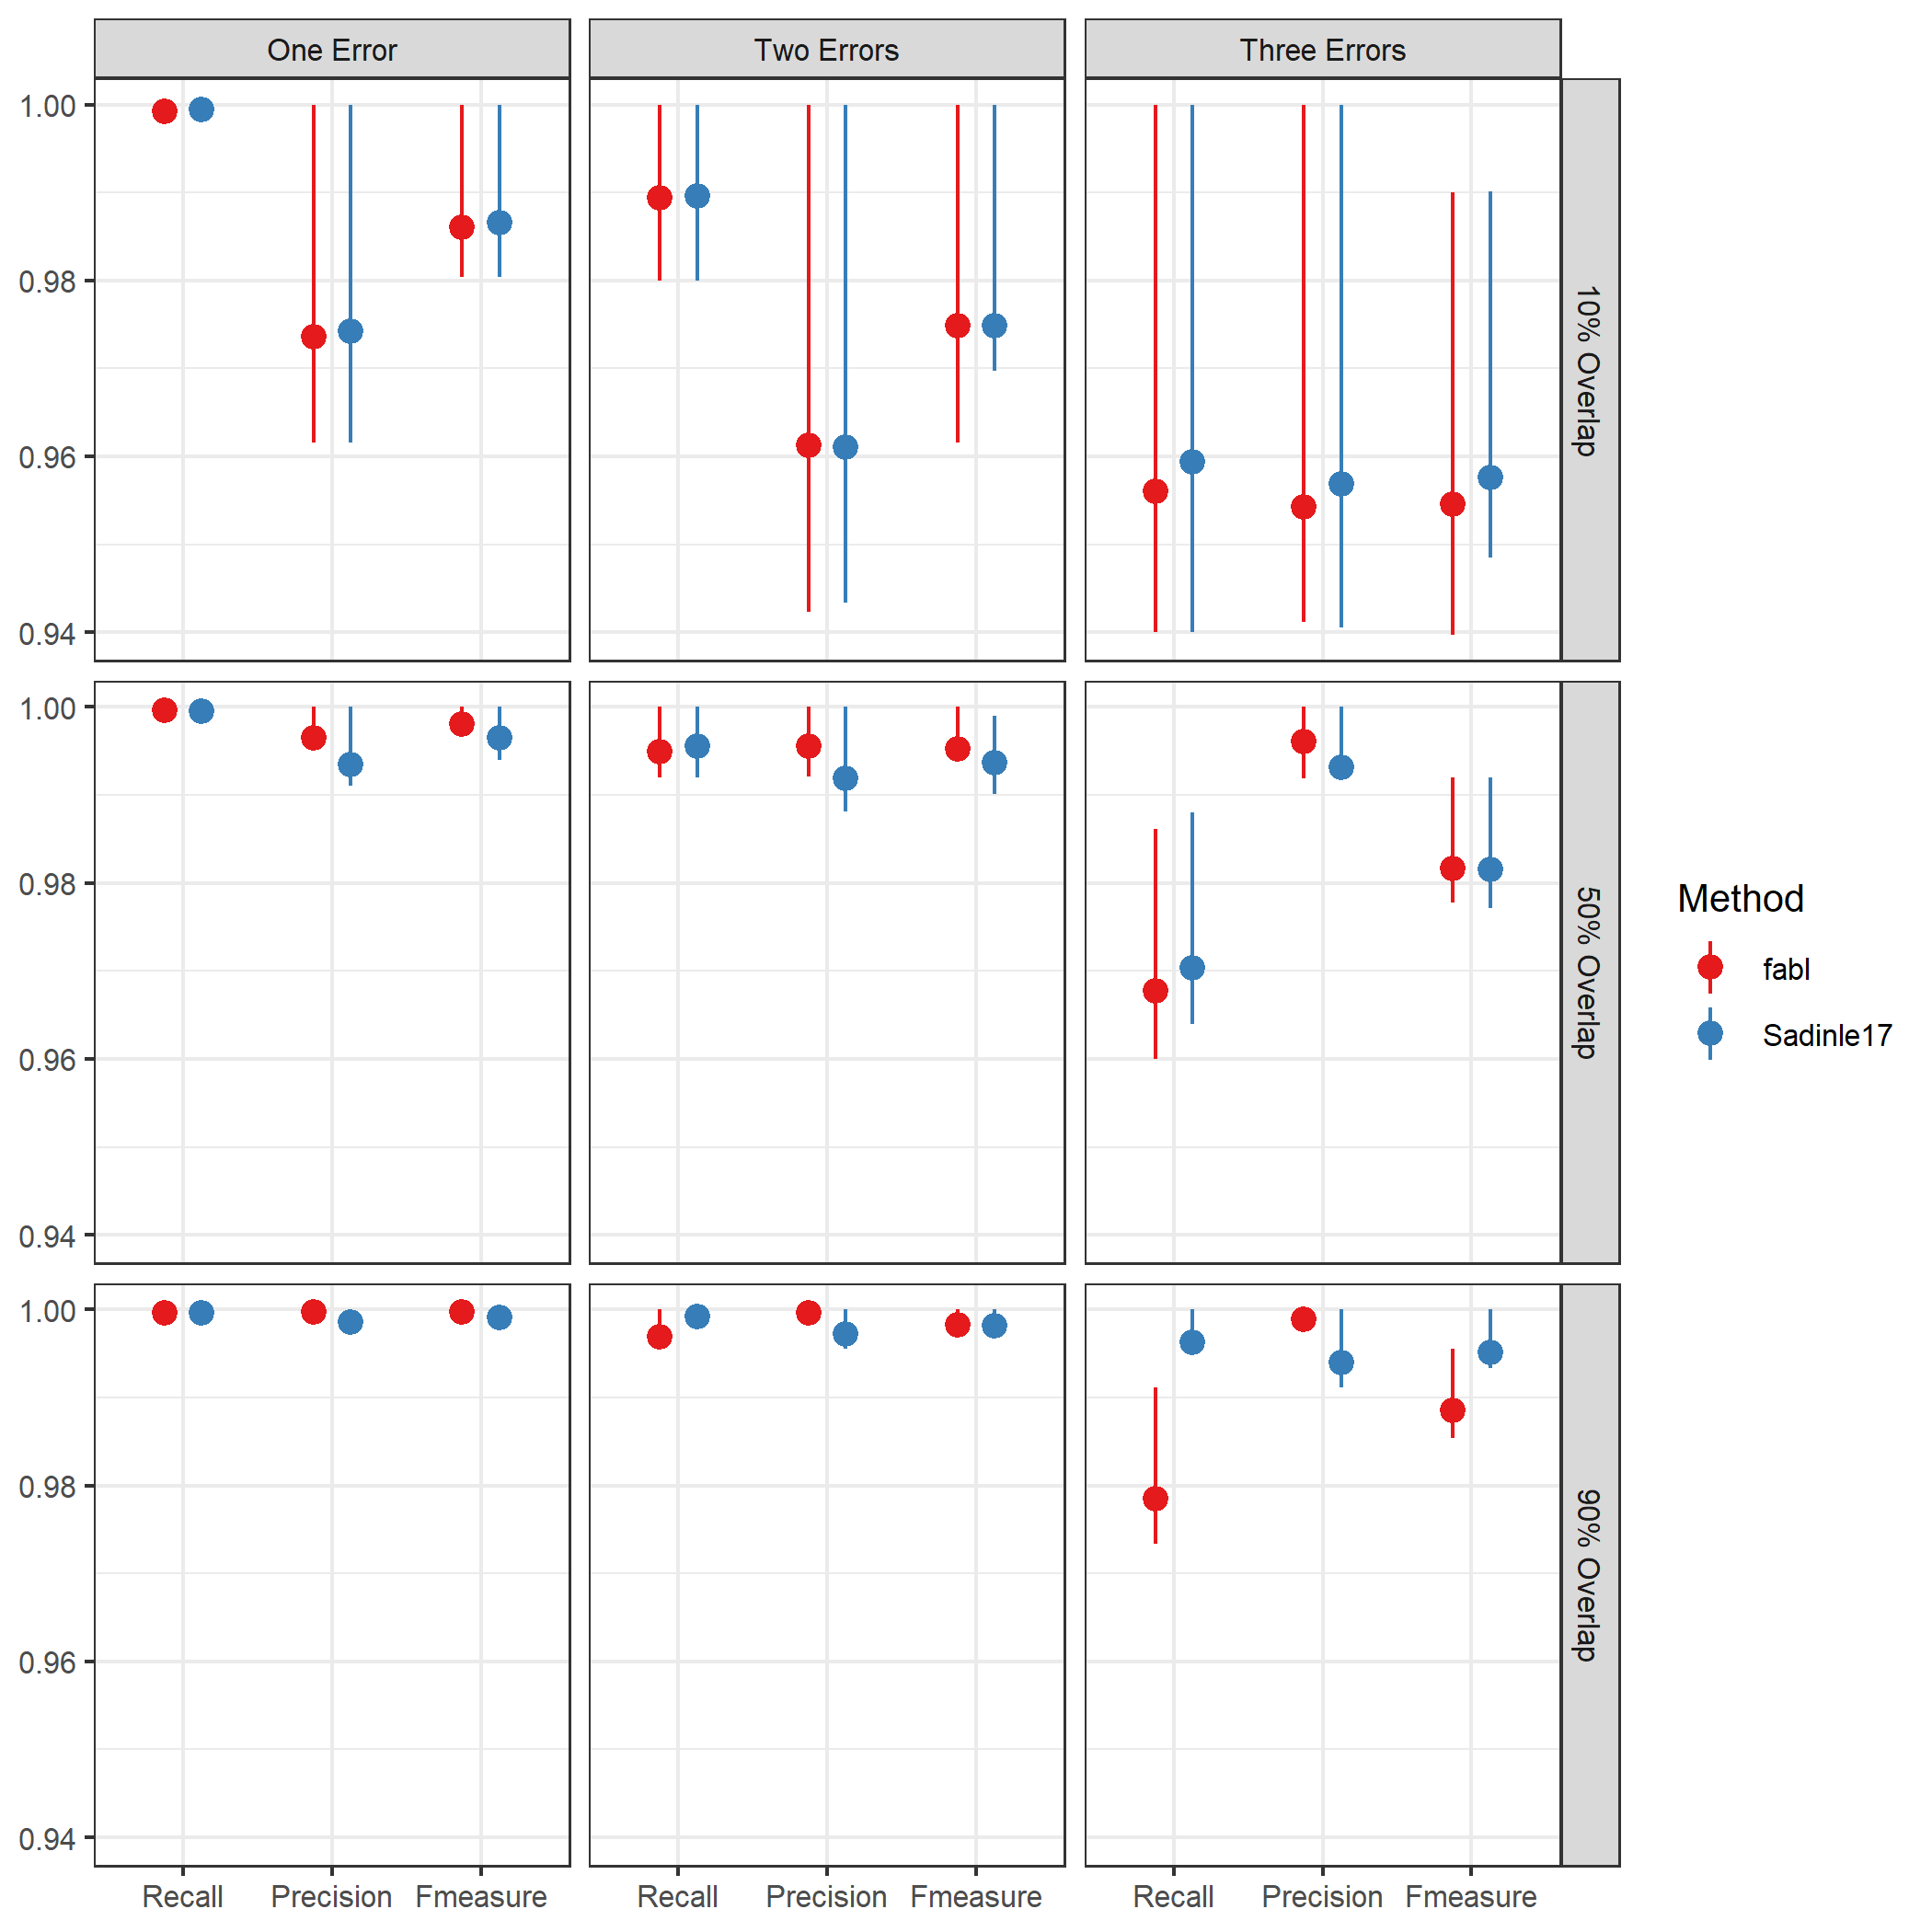
\includegraphics[width=29.17in]{../notes/figures/sadinle_sim_plot} \end{center}

\hypertarget{simulation-study-2---speed}{%
\section{Simulation Study 2 - Speed}\label{simulation-study-2---speed}}

To demonstrate speed, we generate comparison vectors from pre-specified
distributions so that we can easily increase the size of the linkage
problem. Distributions are meant to emulate the behavior of similarity
scores across first name, last name, and day, month, and and year of
birth, with 1 indicating an exact match on a particular field and 0
indicating a nonmatch. We simulate these data for different values of
\(n_A\) and \(n_B\), and compare the run-time of \texttt{parlr} against
\texttt{BRL}. Note that the number of unique patterns \(P\) is bounded
above by \(2^5 = 32\), a bound which is consistently attained in the
larger simulations.

We see that at low data size, \texttt{BRL} outperforms, but that
\texttt{parlr} is significantly faster at handling larger data. In
particular, run-time for \texttt{BRL} seems to grow quadratically (or
linearly with the size of both \(A\) and \(B\)) while run-time for
\texttt{parlr} seems to grow linearly (in the size of \(B\)).

\begin{table}[ht]
\centering
\begin{tabular}{rrr}
  \hline
 & m & u \\ 
  \hline
fname\_0 & 0.05 & 0.99 \\ 
  fname\_1 & 0.95 & 0.01 \\ 
  lname\_0 & 0.05 & 0.99 \\ 
  lname\_1 & 0.95 & 0.01 \\ 
  day\_0 & 0.05 & 0.97 \\ 
  day\_1 & 0.95 & 0.03 \\ 
  month\_0 & 0.05 & 0.92 \\ 
  month\_1 & 0.95 & 0.08 \\ 
  year\_0 & 0.05 & 0.93 \\ 
  year\_1 & 0.95 & 0.07 \\ 
   \hline
\end{tabular}
\end{table}

\begin{center}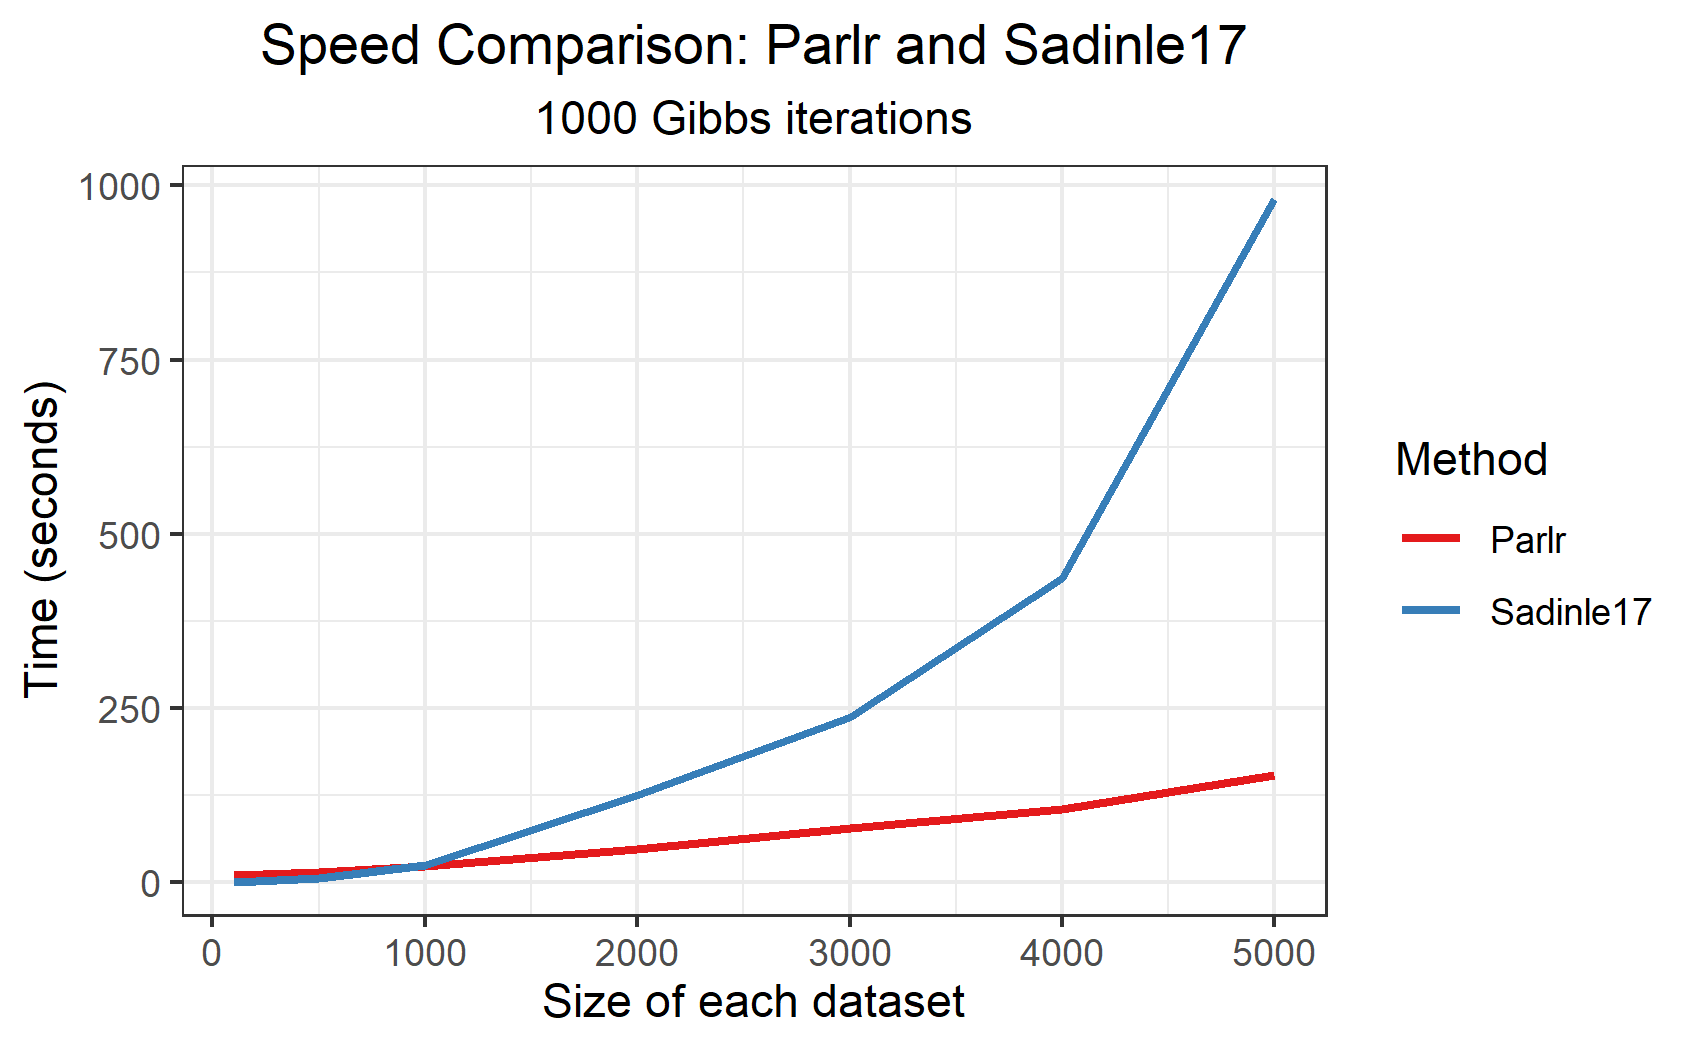
\includegraphics[width=23.6in]{../notes/figures/sadinle_speed_plot} \end{center}

The above discussion suggests that for fixed \(n_B\), computation time
should remain mostly constant with growing \(n_A\). Simulation study
suggests that this is true. In the plot below, fixing \(n_B = 500\), we
see linear growth for the run-time under \texttt{BRL} as \(n_A\)
increases, with much more static run-time under \texttt{parlr}. The
slight increases in run-time that we do see are due primarily to the
hashing step, which again can be run in parallel for large data.

\begin{center}
\includegraphics[width=29.17in]{../notes/figures/speed_plot_fixed_nB} \end{center}

We note here that \texttt{BRL} is coded in C, which makes for unfair
comparison against \texttt{parlr}, currently only built in R.
Additionally, although \texttt{parlr} is amenable to parallelization,
this simulation was run on a single core. Running \texttt{parlr} in C++
with paralellization for the hashing step and sampling the matching
status of the record pairs should lead to even more drastic results.

\hypertarget{data-analysis}{%
\section{Data Analysis}\label{data-analysis}}

the country of El Salvador was immersed in civil war from 1980 to 1991,
and throughout the time, several organizations attempted to document
casualties of the conflict. When estimating the total number of
casualities, one cannot simply sum the numbers recorded by each
organization, as it is likely that the same individuals are recorded in
multiple casuality lists. To obtain a more accurate estimate of the
casualties then, we follow Sadinle's 2017 paper and link records of El
Salvadoran civilian casualties from two sources: El Rescate - Tutela
Regal (ERTL) and the Salvadoran Human Rights Commission (CDHES, by its
acronym in Spanish). The ERTL dataset consists of digitized reports that
had been published throughout the conflict. The CDHES dataset consists
of casualties that had been reported directly to the organization, and
later digitized.

There are several challenges with working with such data. Firstly, both
datasets have been automatically digitized, which inherently leads to
some degree of typographical error. Secondly, the CDHES records are all
second hand accounts reported by individuals, which can result in
additional errors. Lastly, the only fields recorded are given name, last
name, date of death, and place of death; it is relatively common for a
parent and child to share the same given name, resulting in
indistinguishable records for two different individuals. This last point
nearly breaks the above mentioned assumption that there are no
duplicates within files, and reveals a key difference between
\texttt{BRL} and our proposed method.

We only utilized records with nonmissing entries for given and last
name, results in \(n_A = 4420\) files in CHDES and \(n_B = 1323\) files
in ERTL. The names were standardized to account for common misspellings
in the Spanish language, and then compared using a modified Levenstein
distance to account for the fact that second names are often ommited.
Place of birth is recorded by municipality and department within that
municipality; however, since department was missing in 95\% of records
in CHDES and 80\% of records in ERTL, we excluded it from our linkage
process. Thus we conduct linkage using given name, last name,
municipality, and day, month, and year of death. We again use flat
priors for the \(\mathbf{m}\) and \(\mathbf{u}\) parameters, but use
2000 Gibbs iterations with 200 discarded as burn-in to mirror the
implementation in Sadinle 2017.

\hypertarget{discussion}{%
\section{Discussion}\label{discussion}}

\end{document}
